\section{Evaluation}
\subsection{Homogenity of $B$}
The results of the measurement of the homogenity of the magnetic field $B$ 
without applying the modulation are plotted in figure 
\ref{fig:b_height}. As one can see, a good working point is defined for $z = -2$ cm, since 
this is close to the midpoint of the observed plateau. The existence of the plateau indicates the homogenity 
of the field, which is a necessary foundation for the further analysis.
\begin{figure}[H]
    \centering
    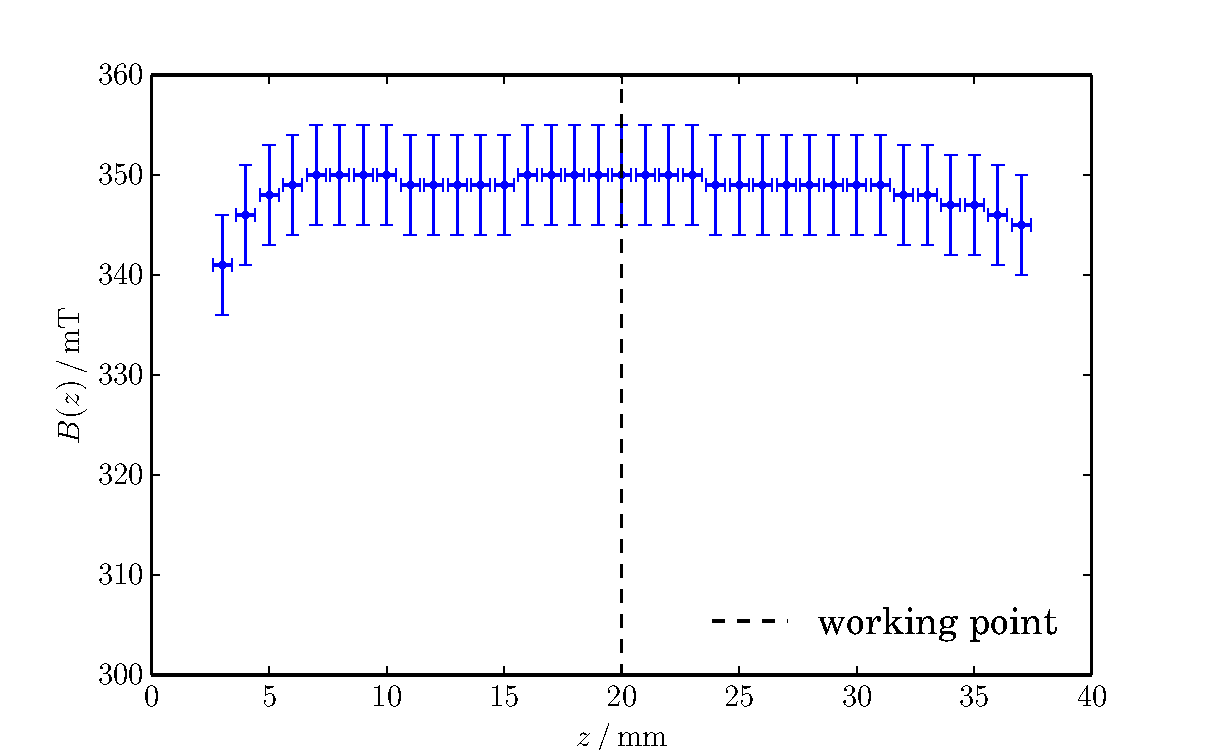
\includegraphics[width=1.0\textwidth]{figures/b_height.pdf}
    \caption{   
        Measurement of the homogenity of the unmodulated magnetic field $B$ in the vertical direction $z$. 
        The appied current is $I = 2.62$ A. As we observe a plateau between $z = 7$ mm and $z = 31$ mm, 
        we define the working point for the further experiments for $z = 20$ mm.
        For measured values, refer to table \ref{tab:b_height}.
        }
    \label{fig:b_height}
\end{figure}
\FloatBarrier


\subsection{Dependency $B(I)$}
Measuring the magnetic fields of the main coil for different currents yielded two 
important results, which can be observed in figure \ref{fig:b_I}:
\begin{itemize}
    \item
        In the regime $I < 3$ A, $B(I)$ behaves linear. We calculated fit parameters 
        for a least square fit using the corresponding routine 'numpy.polyfit'\ref{scipy} for 
        a first degree polynome $f(I) = p_0 I + p_1$ for the pairs $(I, B(I))$, $I \le 3.36$ A. 
        The resulting parameters $p_0$ and $p_1$ with covariance matrix are given by:
        \begin{align}
            p_0 &= 129 \pm 3 \mT / \A\\
            p_1 &= 16 \pm 7 \mT\\
            \mathrm{cov}(p_i, p_j) &= 
            \begin{pmatrix}
                11.1\frac{\mT^2}{\A^2} &-21.5\frac{\mT^2}{\A} \\
                -21.5\frac{\mT^2}{\A} &51.0\mT^2 \\
            \end{pmatrix} 
            \, \mathrm{}
        \end{align}
        The relative error 
        \begin{equation}
            \frac{\Delta p_0}{p_0} = 3 / 129 \approx 2\%
        \end{equation}
        indicates the linear behaviour in the chosen regime which is expected from the 
        graphical analysis. 
    \item
        We observe a non-linear behaviour for $I > 3$ A. However, this regime is 
        not reached during the other measurements, so that we relinquish the further analysis. 
\end{itemize}
\begin{figure}[H]
    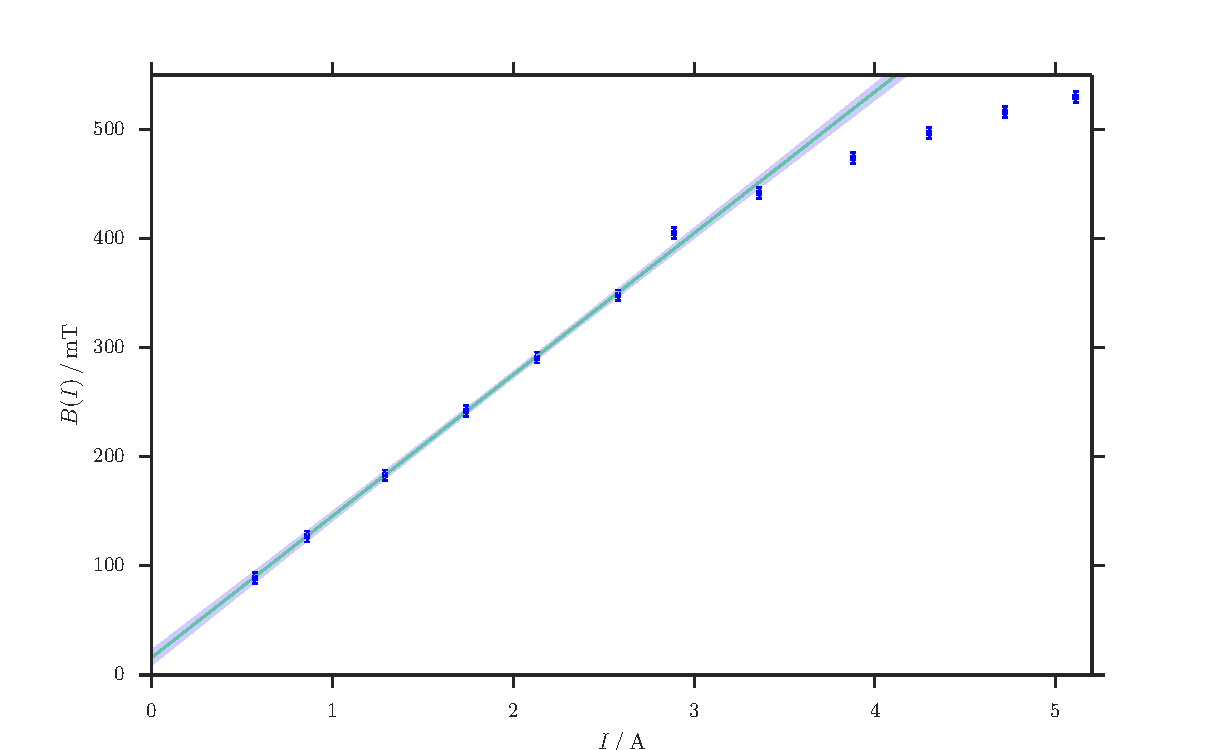
\includegraphics[width=\textwidth]{figures/b_I.pdf}
    \caption{   
        Measurement of magnetic field $B$ of the main coil depending on the applied current 
        $I$ at the working point $z = 20$ mm. The error bars corresponding 
        to the uncertainties $\Delta I = 0.01$ A 
        and $\Delta B = 5$ mT are plotted but visibly very small at this scale. 
        The line is showing the least square fit for $f(I) = p_0 I + p_1$. The 
        lighter shade indicates the uncertainties calculated from the parameters 
        and the covariance matrix. 
        The measured values are shown in table \ref{tab:b_I}.
        }
    \label{fig:b_I}
\end{figure}


\subsection{Direct measurement of $f_r$}
\subsubsection{Calculating magnetic moments and gyromagnetic ratios}





\subsubsection{Comments on the errors}
The fine tuning becomes somewhat useless, as the uncertainty of the current, given by the last 
significant digit is much higher then the difference between 'no absorption seen' and 
'absorption observed'. The drift of the current over time is clearly connected to the developement 
of heat in the coil, which in turn raises the resistance. Due to the high sensitivity of the absorption 
to small changes in $I$ we assume that this drift might be one of the reasons for not finding 
a stable and equidistant signal as expected in the theory section. 





\subsection{Lock-in method}
\paragraph{The reasons for the failure} 
of the Lock-in method remain unclear. Apart from some possible severe 
failure in setting up the experiment, which we tried to prevent by several 
controls as well as trail-and-error manipulation of the parameters used, 
we name the very unstable electronics. From the previous measurements, it was 
already clear that the underlying magnetic field was not very stable, leading 
to an absorption signal very unstable in time. Thus, integrating this signal 
might not lead to the desired amplification over the underlying noise. 

